\section{Zufallsprozesse \formelbuch{165-7}}
\begin{minipage}{10.3cm}
	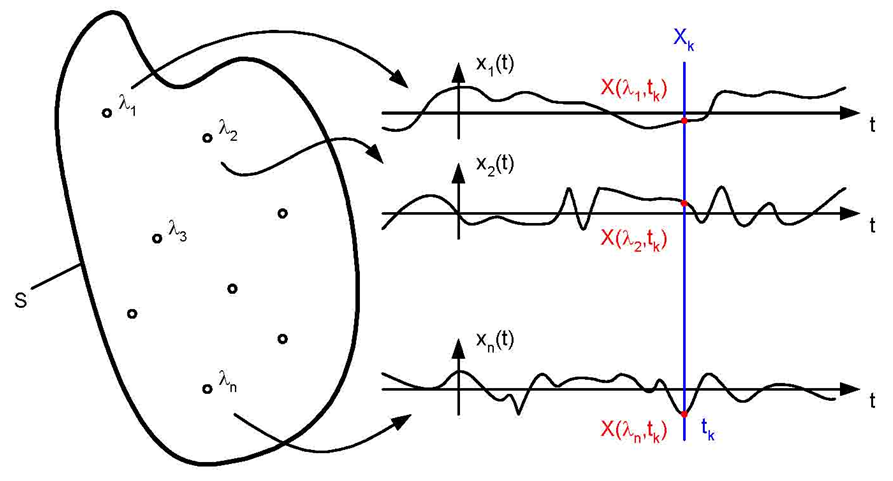
\includegraphics[width=10cm]{../NaT2/bilder/07_zufallsprozess.png}
\end{minipage}
\begin{minipage}{8.5cm}
	Bei einem \textbf{Zufallsprozess} wird jedem \textbf{Ergebnis} \boldmath$\lambda$ aus 
	dem \textbf{Ergebnisraum} $S$ eine \textbf{deterministische} \textbf{Funktion} $x(\lambda, t)$
	\unboldmath zugewiesen. \\
	Zufallsprozesse beschreiben eine deterministische Zeitfunktion ausgelöst durch ein Ergebnis eines
	Zufallsexperiments. \\
	Zeitlich \textbf{zufällig ablaufende Funktionen} können ebenfalls als \textbf{deterministische} Funktionen 
	\textbf{aufgefasst} werden, bei denen der Beobachter nie weiss, welche Funktion $x_\lambda(t)$ konkret
	vorliegt.	\\ \\
	Zum Vergleich: Bei Zufallsvariablen wird jedem Elementarereignis eine Zahl zugewiesen. 
\end{minipage} 
\vspace{0.5cm} \\
Beispiele von Zufallsprozessen:
\begin{itemize}
  \item \textbf{Binäre Datenquelle:} Das auftreten einer $1$ oder $0$ (Ergebnis $\lambda$) ist
  zufällig, jedoch sind die dazugehörigen Pulsformen $x(\lambda_0, t)$ und $x(\lambda_1, t)$
  bekannt.
  \item \textbf{Ethernet-Paket:} Da die Paketlänge $1518$ Bytes beträgt ist der Ergebnisraum $S$
  endlich und beinhaltet alle möglichen Bitkombinationen der Länge von $1518$ Bytes. Das Auftreten
  der jeweiligen Bitfolgen ist zufällig, jedoch ist dann der zeitliche Verlauf der jeweiligen
  Pulsformen vorbestimmt.
  \item \textbf{Manchester-Puls mit Rauschen:} Am Empfänger ist den Bitpulsen \textbf{thermisches Rauschen}
  überlagert. Da man den zeitlichen Verlauf der Rauschspannung nicht vorhersagen kann, existiert
  eine \textbf{unendliche Anzahl Ergebnise} $\lambda$. \\
  Eine deterministische Berechnung des zeitlichen Verlaufs ist nicht möglich, jedoch kann man die
  \textbf{statistischen Eigenschaften} der Rauschquellen aufgrund des physikalischen Modells exakt berechnet
  werden.
\end{itemize}

\skriptsubsection{Statistische Mittelwerte (Scharmittel)}{166-7.3.B}
Die statistischen Mittelwerte sind eine Funktion der Zeit $t$, da es sich um Mittelwerte über das
Ensemble (ganzer Ergebnisraum) handelt. Hierbei werden alle deterministischen Funktionen zu einem
bestimmten Zeitpunkt $t$ gemittelt. 

\renewcommand{\arraystretch}{1.4}
\begin{tabular}[c]{ p{3.5cm}  p{14.5cm}  }
	\textbf{Erwartungswert}: 	&  $\mu_{X}(t) = E\left[X(t)\right] =
          \int\limits_{-\infty}^{+\infty} x \cdot f_{X}(x;t)\;dx$ \\
   	\textbf{Autokorrelation}: 	& 	$R_{XX}(t_{1},t_{2}) = E\left[X(t_{1})X(t_{2})\right] =
          \int\limits_{-\infty}^{+\infty} \int\limits_{-\infty}^{+\infty} 
            x_{1} \cdot  x_{2}\cdot f_{X}(x_{1},x_{2};t_{1},t_{2})\;dx_{1} \;dx_{2}$ \\
	\textbf{Autokovarianz}:		&  $C_{XX}(t_{1},t_{2}) =
          E\left[ \left( X(t_{1})-\mu_{X}(t_{1})\right) \cdot
                  \left( X(t_{2})-\mu_{X}(t_{2})\right) \right] =
          R_{XX}(t_{1},t_{2}) - \mu_{X}(t_{1}) \cdot \mu_{X}(t_{2})$	
\end{tabular}
\renewcommand{\arraystretch}{1}

\skriptsubsection{Zeitliche Mittelwerte (Zeitmittel)}{168-7.3.D}
Hierbei werden die jeweiligen deterministischen Funktionen (Musterfunktionen) zeitlich gemittelt.
Wird das zeitliche Mittel über den gesamten Zufallsprozess berechnet, so handelt es sich bei den
zeitlichen Mittelwerten um \textbf{Zufallsvariablen}, d.h. die folgenden zwei Ausdrücke sind
abhängig davon (darum Index $_i$), welche Funktion genutzt wird.

%\renewcommand{\arraystretch}{1.4}
\begin{tabular}[c]{ p{4cm}  p{14.5cm}  }
	\textbf{Mittelwert}: 	&  
	$\overline{x_{i}} = \left\langle x_{i}(t) \right\rangle = 
           \lim\limits_{T \rightarrow \infty}
             \frac{1}{T} \int\limits_{-\frac{T}{2}}^{+\frac{T}{2}} x_{i}(t) \; dt$ \\
   	\textbf{Autokorrelation}: 	& 	
   	$\overline{R}_{X_{i}X_{i}}(\tau) = \left\langle x_{i}(t) \cdot x_{i}(t+\tau) \right\rangle = 
           \lim\limits_{T \rightarrow \infty}
             \frac{1}{T} \int\limits_{-\frac{T}{2}}^{+\frac{T}{2}} x_{i}(t) \cdot x_{i}(t + \tau) \; dt$\\
    \multicolumn{2}{l}{Falls der \textbf{Prozess stationär} ist gilt zudem: } \\
	\textbf{Mittelwert}: 	&  
	$E[\overline{x}] = 
           \lim\limits_{T \rightarrow \infty}
             \frac{1}{T} \int\limits_{-\frac{T}{2}}^{+\frac{T}{2}} E[x(t)] \; dt = 
             \frac{1}{T} \int\limits_{-\frac{T}{2}}^{+\frac{T}{2}} \mu_{X} \; dt = \mu_{X}(t)$  \\
   	\textbf{Autokorrelation}: 	& 	
   	$E[\overline{R}_{XX}(\tau)] = 
           \lim\limits_{T \rightarrow \infty}
             \frac{1}{T} \int\limits_{-\frac{T}{2}}^{+\frac{T}{2}} E[x(t)x(t+\tau)] \; dt =
             \frac{1}{T} \int\limits_{-\frac{T}{2}}^{+\frac{T}{2}} R_{XX}(\tau) \; dt = R_{XX}(\tau)$\\
\end{tabular}
\renewcommand{\arraystretch}{1}

\skriptsubsection{Stationarität}{167-7.3.C}
Ein stationärer Prozess verändert seine statistischen Eigenschaften über die
Zeit nicht. Wenn ein Prozess ergodisch ist, ist er auch stationär (nicht
umgekehrt).\\

\subsubsection{Streng Stationär (SSS - Strict Sense Stationary)}
% TODO genaue beschreibung streng, schwach stationär
Bei einem streng stationären Prozess bleiben die n-dimensionale WSK-Dichten über die
Zeit konstant. D.h. die \textbf{statistischen Eigenschaften} und somit auch die WSK-Dichten sind zu 
\textbf{allen Zeitpunkten dieselben}.
$$ f_X(x_1, x_2, \ldots, x_n; t_1, t_2, \ldots, t_n) =
		f_X(x_1, x_2, \ldots, x_n; t_1+c, t_2+c, \ldots, t_n+c) \qquad \forall (c,n \in
		\mathbb{R})$$
% Es gelten folgende Beziehungen: \\
% $$E[X(t)] = \mu_{X} \qquad \qquad
% R_{XX}(t_{1},t_{2}) = R_{X}(\tau),\quad \text{ mit } \tau = t_{2} - t_{1} \qquad \qquad
% C_{XX}(t_{1},t_{2}) = R_{X}(\tau) - \mu_{X}^{2}$$ 

\subsubsection{Schwach Stationär (WSS - Wide Sense Stationary) - Stationarität 2. Ordnung}
Bei einem schwach stationären Prozess sind die statistischen Eigenschaften zwar
\textbf{nicht zu jedem Zeitpunkt die selben}, jedoch sind sie \textbf{nicht} von einem \textbf{absoluten} Zeitpunkt, sondern
von der \textbf{Differenz} ($\tau$) \textbf{zweier Zeitpunkte} ($t_1, t_2$) abhängig.  \\ 
$$ f_X(x_1, x_2; t_1, t_2) = f_X(x_1, x_2; t_1+c, t_2+c) \qquad \forall (c \in
		\mathbb{R})$$
%Zudem gilt:\\
\renewcommand{\arraystretch}{1.4}
\begin{tabular}[c]{ p{3.3cm}  p{6.5cm} p{8cm} }
	\textbf{Mittelwert}: 	&  $E[X(t)] = \mu_{X}(t) = \text{const.}$  
							& bleibt über die ganze Zeit konstant\\ 
	\textbf{quad. Mittelwert}: 	&  $E[X^{2}(t)] = R_{X}(0)$  \\ 
	\textbf{Autokorrelation}: 	& 	$R_{XX}(t_{1},t_{2}) = R_{X}(\tau)$
	& \multirow{2}{8cm}{nur \textbf{abhängig} von der \textbf{Zeitdifferenz} $(\tau = t_2 - t_1)$ und \textbf{nicht direkt} von
	 der \textbf{Zeit} $t$} \\
	 \textbf{Autokovarianz}:		& $ C_{XX}(t_{1},t_{2}) = R_{X}(\tau) - \mu_{X}(t)^{2} = C_{XX}(\tau)$ \\
\end{tabular}
\renewcommand{\arraystretch}{1}
 
Bei einem Zufallsprozess handelt es sich immer um ein WSS-Prozess, sobald der Erwartungswert
für jede Zeit $t$ konstant bleibt und die Autokorrelationsfunktion nur eine Funktion von $\tau$ ist,
d.h. beide statistischen Kennwerte bzgl. einer zeitlichen Verschiebung unabhängig sind.    
Jeder streng stationäre Prozess ist auch schwach stationär, aber nicht umgekehrt. 
        
%   \item Zwei Zufallsprozesse heissen Verbund-schwach-station\"ar, wenn jeder Prozess f\"ur sich 
%         schwach-station\"ar ist und zudem gilt:  
%         \begin{itemize}
%           \item[$\circ$] $R_{XY}(t_{1},t+\tau) = E[X(t)Y(t+\tau)] = R_{XY}(\tau)$ 
%         \end{itemize} 
%   \item Dann gilt auch:
%   \begin{itemize}
%      \item[$\circ$] $C_{XY}(\tau) = R_{XY}(\tau) - \mu_{X} \mu_{Y}$
%   \end{itemize} 
% \end{itemize} 

%TODO verbund schwach stationär

\skriptsubsection{Ergodizität}{168-7.3.D}
Ein stationärer Prozess ist zudem noch ergodisch, wenn \textbf{\textcolor{red}{alle} zeitlichen
Mittelwerten} (Zeitmittelwert und zeitlich gemittelte Autokorrelation) den \textbf{statistischen
Mittelwerten} (Erwartungswert und statistisch gemittelte Autokorrelation)
\textbf{entsprechen}. Jeder ergodische Zufallsprozess ist auch stationär, aber
nicht umgekehrt.
%\hspace{2cm} \textbf{Zeitmittel = Scharmittel}\\


	\begin{minipage}{5cm}
		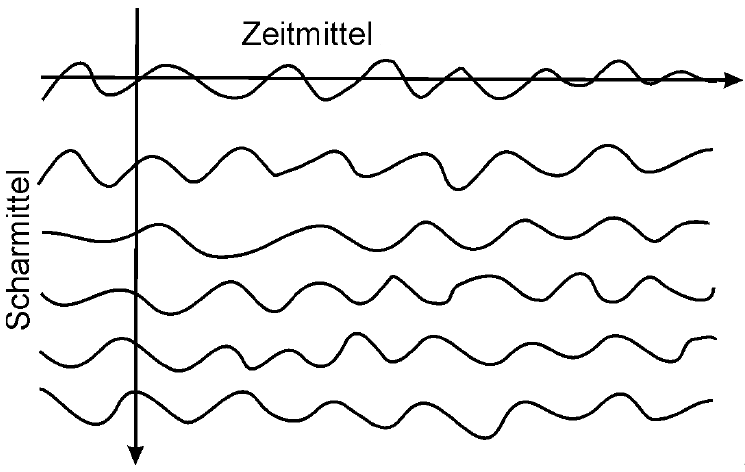
\includegraphics[width=4.7cm]{../NaT2/bilder/07_zeit-scharmittel.png}
  	\end{minipage}
	\begin{minipage}{13.5cm}
	\begin{tabular}{llll}  
    	Statistische MW $ \left\{
    	\begin{array}{ccc}
       		E[X(t)] & = & \overline{x}_i \\
       		R_{XX}(\tau) & = & \overline{R}_{X_iX_i}(\tau)
       \end{array}
		\right\} $
		Zeitliche MW (\textbf{const. für alle i})
    \end{tabular} \\

	\begin{tabular}{ll}
  		\multicolumn{2}{l}{Nur bei ergodischen Prozessen gilt zwingend:} \\
      $E[X(t)] = \overline{x} = \left\langle x(t) \right\rangle$ & DC-Level \\
      $E[X(t)]^{2} = (\overline{x})^{2} = \left\langle x(t) \right\rangle^{2}$ & DC-Leistung \\
      $E[X^{2}(t)] = R_{XX}(0) = \overline{x^{2}} = 
                     \left\langle x^{2}(t) \right\rangle $ & Gesamtleistung \\
      $\sigma_{X}^{2}(t) = \left\langle x^{2}(t) \right\rangle 
                           - \left\langle x(t) \right\rangle^{2}$ & AC-Leistung \\
      $\sigma_{X}(t) = \overline{\sigma}_{X}$ & RMS-Level (Effektivwert) des AC-Signals\\
    \end{tabular}
  	\end{minipage}


\subsection{Vergleich Stationär - Ergodisch}
\subsubsection{Mückenschwarm}
\textbf{Ergodisch:} Fliegen alle Mücken zusammen in einem Schwarm, so fliegt jede Mücke über die
ganze Zeit gemittelt (Zeitmittel) so schnell wie der ganze Schwarm im Mitel (Scharmittel), ansonsten
würde der Schwarm nicht zusammenhalten können. \\
\textbf{Stationär:} Ist eine Mücke krank und kann mit dem Schwarm nicht mithalten, so fliegt sie
alleine und v.a. langsamer. Somit ist ihre Durchschnittsgeschwindigkeit (Zeitmittel) nicht gleich
derjenigen des Schwarms (Scharmittel), also kommt sie später am Ziel an. \\
\textbf{Weder noch:} Fliegen die Mücken nach dem Start immer langsamer, so ist die
durchschnittliche Geschwindigkeit des Schwarms (Scharmittel) nicht konstant.

\subsubsection{Schulnoten}
\textbf{Ergodisch:} Alle Schüler müssten dieselbe Zeugnisnote (Zeitmittel) haben und zudem müsste
diese Note jeweils auch dem Klassenschnitt (Scharmittel) der einzelnen Prüfungen entsprechen. \\
\textbf{Stationär:} Der Klassenschnitt (Scharmittel) ist bei jeder Prüfung gleich, jedoch gibt es
unterschiedlich starke Schüler mit unterschiedlichen Zeugnisnoten (Zeitmittel). \\
\textbf{Weder noch:} Der Klassenschnitt (Scharmittel) ist immer unterschiedlich.

\subsubsection{Thermisches Widerstandsrauschen} 
Dies ist bei gleichbleibender Temperatur \textbf{ergodisch}.


\skriptsubsection{Korrelationen und Leistungsspektren}{169-7.4}
Formeln in diesem Abschnitt gelten für \textbf{stationäre} Prozesse. \\

\renewcommand{\arraystretch}{1.6}
\begin{tabular}[c]{ p{4cm}  p{6cm} p{7.5cm} }
	\textbf{Autokorrelation}: 	&  
	$R_{XX}(\tau) = E[X(t)X(t+\tau)]$ \\
  	&	$\mid \! R_{XX}(\tau) \! \mid \leq R_{XX}(0) = E[X^{2}(t)]$ 
	& $R_{XX}(-\tau) = R_{XX}(\tau) \quad$ (gerade)\\
  \textbf{Kreuzkorrelation}: 	& 	
 	$R_{XY}(\tau) = E[X(t)Y(t+\tau)]$  
	& $R_{XY}(-\tau) = R_{YX}(\tau) \quad$ (Reihenfolge Indizes!) \\
	& $|R_{XY}(\tau)| \leq \frac{1}{2} \left[ R_{XX}(0)+R_{YY}(0)\right] $
	& $|R_{XY}(\tau)|  \leq \sqrt{R_{XX}(0)R_{YY}(0)}$ \\
   \textbf{Autokovarianz}: 	&  
	\multicolumn{2}{l}{$C_{XX}(\tau) = E\!\left[ \left( X(t)      - E[X(t)]      \right) \cdot
                                  \left( X(t+\tau) - E[X(t+\tau)] \right) \right] =
                        R_{XX}(\tau) - \mu^{2}_{X} $} \\
   	\textbf{Kreuzkovarianz}: 	& 	
   	\multicolumn{2}{l}{$C_{XY}(\tau) = E\!\left[ \left( X(t)      - E[X(t)]      \right) \cdot
                                  \left( Y(t+\tau) - E[Y(t+\tau)] \right) \right] =
                        R_{XY}(\tau) - \mu_{X}\mu_{Y} $}\\
    & \multicolumn{2}{l}{Zufallsprozesse bezeichnet man als zueinander
                        \textbf{unkorreliert}, wenn $C_{XY}(\tau) = 0$}
\end{tabular}
\renewcommand{\arraystretch}{1}

\skriptsubsubsection{Spektrale Leistung}{170-7.4.E,F}
Autokorrelationsfunktion $R_{XX}(\tau)$ und Leistungsspektraldichte $S_{XX}(\omega)$ bilden ein
Fourier-\textbf{Transformationspaar}. \\ Die Leistungsspektraldichte kann als \textbf{mittlere Leistung pro Frequenzband }aufgefasst werden, sie ist
wie folgt definiert:                             
        $$ E\left[ \lim\limits_{T \rightarrow \infty} \frac{1}{T} \cdot \mid\!
        X(\omega) \!\mid^{2}\right] = \int\limits_{-\infty}^{+\infty}
        R_{XX}(\tau) \cdot e^{-j\omega\tau} \; d\tau = \boxed{S_{XX}(\omega)
        \qquad \IFT \qquad R_{XX}(\tau)} = \frac{1}{2\pi}
        \int\limits_{-\infty}^{+\infty}S_{XX}(\omega) \cdot e^{j\omega\tau} \;
        d\omega$$ $S_{XX}(\omega)$ ist rein reell und $\geq 0$. \\
Kreuzkorrelationen ($R_{YX}(\tau), R_{XY}(\tau)$) und Kreuz-Spektraldichten ($S_{YX}(\tau),
S_{XY}(\tau)$) bilden ein Fourier-Transformationspaar.
\begin{center}
	$R_{YX}(\tau) \FT S_{YX}(\omega) \qquad \qquad R_{XY}(\tau) \FT S_{XY}(\omega)$
\end{center}



\skriptsubsection{Übertragung von Zufallsprozessen durch LTI-Systeme}{171-7.5}
Ein Zufallsprozess wird durch ein LTI-System übertragen. \hspace{2cm} $Y(t) = L[X(t)] \Rightarrow
Y(t) = h(t) \ast X(t)$ \vspace{0.3cm}\\
\renewcommand{\arraystretch}{1.4}
 \begin{tabular}[c]{ p{2cm}  p{8.5cm} p{8cm} }
	& \textbf{Allgemein} & \textbf{WSS-Prozess} \\
	\textbf{Mittelwert}
		& $\mu_{Y}(t) = h(t) \ast \mu_{X}(t)$
		& $\mu_{Y} = H(0) \mu_{X}$ \\
	\textbf{Auto-korrelation\textcolor{red}{*}}
		& {$R_{YY}(t_{1},t_{2}) = \int\limits_{-\infty}^{+\infty}
		\int\limits_{-\infty}^{+\infty} h(\alpha) h(\beta)
                      R_{XX}(t_{1}-\alpha, t_{2}-\beta) \; d\alpha \; d\beta$}
		& {$R_{YY}(\tau) = \int\limits_{-\infty}^{+\infty}
		\int\limits_{-\infty}^{+\infty} h(\alpha) h(\beta)
                      R_{XX}(\tau+\alpha-\beta) \; d\alpha \; d\beta$} \\
	\textbf{Spektrale Leistung}
		&
		& $\boxed{S_{YY}(\omega)= H^{\ast}(\omega) H(\omega) S_{XX}(\omega)
			= |H(\omega)|^{2} S_{XX}(\omega)}$  \\
\end{tabular}
\renewcommand{\arraystretch}{1} \\
\textcolor{red}{*} = Es ist viel einfacher die Autokorrelation aus der Spektralen Leistung
(Transformationspaar) - anstatt aus diesem höllischen Integral - auszurechnen. \\
Ein WSS-Prozess am Eingang erzeugt auch einen WSS-Prozess am Ausgang.

\skriptsubsection{Spezielle Zufallsprozesse}{172-7.6}
\skriptsubsubsection{Gauss Zufallsprozess}{172-7.6.A}
Bein diesem Prozess ist die \textbf{Zufallsvariable} $X(t_{i})$ zu \textbf{jedem Zeitpunkt} $t_{i}$
\textbf{gaussverteilt}. Bsp.: thermisches Rauschen. \\
Zweidimensionaler Fall (gauss'sche Verbunddichte): 
        $f_{XX}(x_{1},x_{2};t_{1},t_{2}) = \frac{1}{2\pi \sigma_{x_{1}}\sigma_{x_{2}}} \cdot
                                      e^{-\frac{(x_{1}-\mu_{x_{1}})^{2}}{2 \sigma^{2}_{x_{1}}}} \cdot
                                      e^{-\frac{(x_{2}-\mu_{x_{2}})^{2}}{2 \sigma^{2}_{x_{2}}}}$ \\
Für $X(t_{1})$ und $X(t_{2})$ unkorreliert ($C_{XX}(t_{1},t_{2})=0$) gilt:
        $f_{XX}(x_{1},x_{2}; t_{1},t_{2}) = f_{X}(x_{1};t_{1}) \cdot f_{X}(x_{2};t_{2}) $ \\ \\
$\mu_{X}(t)$ und $R_{XX}(t_{1}, t_{2})$ charakterisisieren einen gauss'schen Zufallsprozess
        vollst\"andig. \\
Ist ein gauss'scher Prozess WSS ist er zugleich auch SSS. Zudem ist wird ein gauss'scher
Zufallsprozess $X(t)$ am Ausgang eines LTI Systems $Y(t)$ wiederum gaussisch.

\skriptsubsubsection{Weisses Rauschen}{173-7.6.B}
\begin{center}
	\begin{minipage}{8cm}
		$S_{XX}(\omega) = \dfrac{\eta}{2} \qquad R_{XX}(\tau) = \dfrac{\eta}{2} \cdot \delta(\tau)$ \\ \\
		Beispiel: therm. Rauschen von Widerständen \\
		\textbf{Nimmt} in der Praxis im \textbf{Tera-Hz Bereich ab}!
  	\end{minipage}
	\begin{minipage}{10cm}
		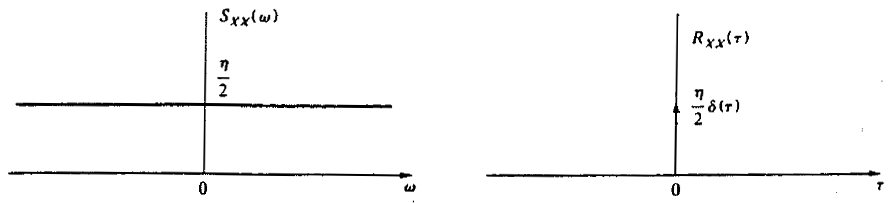
\includegraphics[width=9cm]{../NaT2/bilder/07_weisses_rauschen.png}
  	\end{minipage}
\end{center}

\subsubsection{Farbige Rauschsignale}
\renewcommand{\arraystretch}{2}
\begin{tabular}[c]{ | p{4cm} | p{3.5cm} | p{3cm} | p{6cm} | }
% 	\hline
% 		Weisses Rauschen
% 		& White Noise
% 		& $S_{XX}(\omega) = \dfrac{\eta}{2}$
% 		& \\
	\hline
		\textbf{Bezeichnung (De)}
		& \textbf{Bezeichnung (En)}
		& \textbf{Leist.-Spektrum}
		& \textbf{Anmerkung} \\
	\hline
		Rosa Rauschen
		& Pink Noise
		& $S_{XX}(\omega) = c \cdot \dfrac{1}{\omega}$
		& Testsignal für Tontechnik, wegen konstanter Leistung pro Oktave \\
	\hline
		Braunes/Rotes Rauschen
		& Brown/Red Noise
		&	$S_{XX}(\omega) = c \cdot \dfrac{1}{\omega^2}$
		& \\
	\hline
		Blaues Rauschen
		& Blue Noise
		&	$S_{XX}(\omega) = c \cdot \omega$
		& \\
	\hline
		Violettes Rauschen
		& Purple/Violet Noise
		&	$S_{XX}(\omega) = c \cdot \omega^2$
		& Bsp.: FM Demodulator Noise\\
    \hline
\end{tabular}
\renewcommand{\arraystretch}{1}

\skriptsubsubsection{Bandbeschränktes Rauschen}{174-7.6.C}
\begin{center}
	\begin{minipage}{8cm}
		$S_{XX}(\omega) = \begin{cases}
                      \dfrac{\eta}{2} & |\omega| \leq \omega_B \\
                      0 & |\omega| > \omega_B
                      \end{cases} \\ \\
		R_{XX}(\tau) =  \frac{1}{2\pi} \int\limits_{-\omega_{b}}^{+\omega_{b}}
                                           \frac{\eta}{2}  \cdot e^{j\omega\tau}\; d\tau
                      = \frac{\eta\omega_{B}}{2\pi} \frac{\sin(\omega_{B}\tau)}{\omega_{B}\tau}$
  	\end{minipage}
	\begin{minipage}{10cm}
		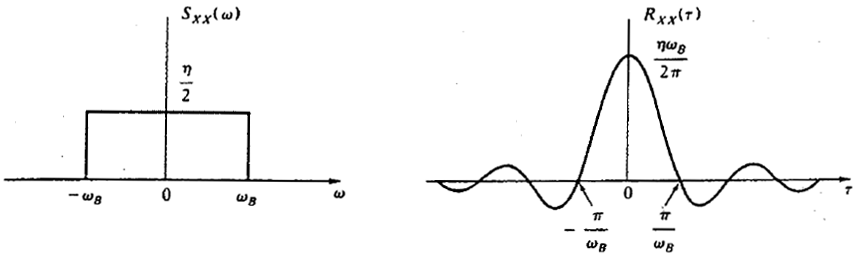
\includegraphics[width=9cm]{../NaT2/bilder/07_bandlimited_whitenoise.png}
  	\end{minipage}
\end{center}

\skriptsubsubsection{Schmalbandiger Zufallsprozess}{174-7.6.D}
\label{schmalbandiger_zufallsprozess}
	\begin{minipage}{9.5cm}
		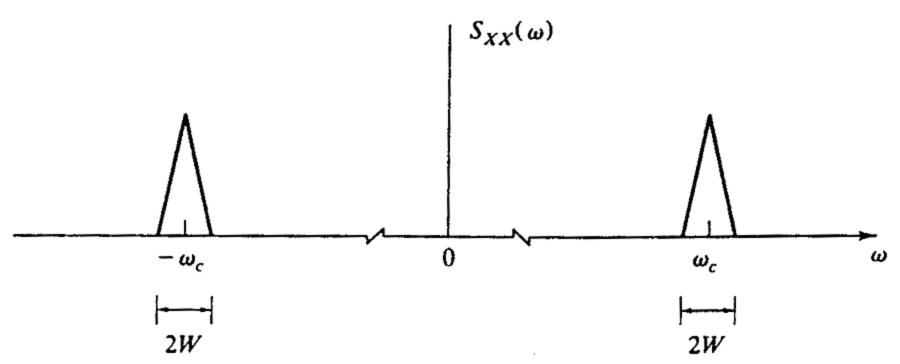
\includegraphics[width=9cm]{../NaT2/bilder/07_schmalbandiger_zufallsprozess.png}
  	\end{minipage}
	\begin{minipage}{8.8cm}
		Hierbei handelt es sich um einen WSS-Prozess mit \textbf{sehr kleiner Bandbreite} $2W$ verglichen mit der
		Mittenfrequenz $\omega_c$. \\
		Dies ist beispielsweise der Fall wenn \textbf{thermisches Widerstandrauschen} durch ein schmalbandiges
		Bandpass gefiltert wird. \\
		Im \textbf{Zeitbereich} manifestiert sich diese Funktion als \textbf{sinusförmiges} Signal mit
		zufälliger Amplitude und Phase. \\
		Bei $X_{c}(t)$ und $X_{s}(t)$ handelt es sich damit um bandbeschr\"anktes Rauschen im Basisband.
  	\end{minipage} \\
	\begin{minipage}{10cm}
		\boldmath$$X(t) = V(t) \cdot \cos \left[ \omega_{c}t + \phi(t) \right]$$ \unboldmath
		$$X(t) = X_{c}(t)\cos\omega_{c}(t) - X_{s}(t)\sin\omega_{c}(t)$$
		$$X_{c}(t) = V(t)\cos\phi(t) \qquad X_{s}(t) = V(t)\sin\phi(t)$$
		$$V(t) = \sqrt{X^{2}_{c}(t) + X^{2}_{s}(t)} \qquad \phi(t) = \arctan \frac{X_{s}(t)}{X_{c}(t)}$$
  	\end{minipage}
	\begin{minipage}{8cm}
		$V(t)$ Enveloppen-Funktion \\ 
        $\phi(t)$ Phasenfunktion. \\
		$X_{c}(t)$ gleichphasiger Anteil \\ 
        $X_{s}(t)$ Quadratur-Anteil        
  	\end{minipage} \\

Eigenschaften von $X_{c}(t)$ und $X_{s}(t)$: \\

\renewcommand{\arraystretch}{1.5}
\begin{tabular}{p{4.5cm} p{4.5cm} p{9cm}}
	$\mu_{X_{c}} = \mu_{X_{s}} = \mu_{X} = 0$
		& $\sigma^{2}_{X_{c}} = \sigma^{2}_{X_{s}} = \sigma^{2}_{X}$
		& $E\left[ X_{c}(t)X_{s}(t) \right]  = 0$ (unkorreliert \& orthogonal) \\
	\multicolumn{3}{c}{$S_{X_{c}X_{c}}(\omega) = S_{X_{s}X_{s}}(\omega)
                   = \left\lbrace
                       \begin{array}{ll}
                         S_{XX}(\omega -\omega_{c}) +S_{XX}(\omega +\omega_{c})
                                        & \mid\!\omega\!\mid \leq W \\
                         0              & \mid\!\omega\!\mid > W \\
                       \end{array} \right. $} \\ 
\end{tabular}
\renewcommand{\arraystretch}{1}

Ist $X(t)$ ein Gauss-Prozess, sind auch $X_{c}(t)$ und $X_{s}(t)$ gaussisch. Dann ist $V(t)$
Rayleigh-verteilt zu jedem Zeitpunkt t und $\Phi(t)$ gleichverteilt ($0..2\pi$) zu jedem
Zeitpunkt t. 
